\documentclass[oneside,12pt]{amsart}

\usepackage{amsmath,amssymb,latexsym,eucal,amsthm,tikz-cd,array,multirow}

%%%%%%%%%%%%%%%%%%%%%%%%%%%%%%%%%%%%%%%%%%%%%
% Common Set Theory Constructs
%%%%%%%%%%%%%%%%%%%%%%%%%%%%%%%%%%%%%%%%%%%%%

\newcommand{\setof}[2]{\left\{ \, #1 \, \left| \, #2 \, \right.\right\}}
\newcommand{\lsetof}[2]{\left\{\left. \, #1 \, \right| \, #2 \,  \right\}}
\newcommand{\bigsetof}[2]{\bigl\{ \, #1 \, \bigm | \, #2 \,\bigr\}}
\newcommand{\Bigsetof}[2]{\Bigl\{ \, #1 \, \Bigm | \, #2 \,\Bigr\}}
\newcommand{\biggsetof}[2]{\biggl\{ \, #1 \, \biggm | \, #2 \,\biggr\}}
\newcommand{\Biggsetof}[2]{\Biggl\{ \, #1 \, \Biggm | \, #2 \,\Biggr\}}
\newcommand{\dotsetof}[2]{\left\{ \, #1 \, : \, #2 \, \right\}}
\newcommand{\bigdotsetof}[2]{\bigl\{ \, #1 \, : \, #2 \,\bigr\}}
\newcommand{\Bigdotsetof}[2]{\Bigl\{ \, #1 \, \Bigm : \, #2 \,\Bigr\}}
\newcommand{\biggdotsetof}[2]{\biggl\{ \, #1 \, \biggm : \, #2 \,\biggr\}}
\newcommand{\Biggdotsetof}[2]{\Biggl\{ \, #1 \, \Biggm : \, #2 \,\Biggr\}}
\newcommand{\sequence}[2]{\left\langle \, #1 \,\left| \, #2 \, \right. \right\rangle}
\newcommand{\lsequence}[2]{\left\langle\left. \, #1 \, \right| \,#2 \,  \right\rangle}
\newcommand{\bigsequence}[2]{\bigl\langle \,#1 \, \bigm | \, #2 \, \bigr\rangle}
\newcommand{\Bigsequence}[2]{\Bigl\langle \,#1 \, \Bigm | \, #2 \, \Bigr\rangle}
\newcommand{\biggsequence}[2]{\biggl\langle \,#1 \, \biggm | \, #2 \, \biggr\rangle}
\newcommand{\Biggsequence}[2]{\Biggl\langle \,#1 \, \Biggm | \, #2 \, \Biggr\rangle}
\newcommand{\singleton}[1]{\left\{#1\right\}}
\newcommand{\angles}[1]{\left\langle #1 \right\rangle}
\newcommand{\bigangles}[1]{\bigl\langle #1 \bigr\rangle}
\newcommand{\Bigangles}[1]{\Bigl\langle #1 \Bigr\rangle}
\newcommand{\biggangles}[1]{\biggl\langle #1 \biggr\rangle}
\newcommand{\Biggangles}[1]{\Biggl\langle #1 \Biggr\rangle}


\newcommand{\force}[1]{\Vert\!\underset{\!\!\!\!\!#1}{\!\!\!\relbar\!\!\!%
\relbar\!\!\relbar\!\!\relbar\!\!\!\relbar\!\!\relbar\!\!\relbar\!\!\!%
\relbar\!\!\relbar\!\!\relbar}}
\newcommand{\longforce}[1]{\Vert\!\underset{\!\!\!\!\!#1}{\!\!\!\relbar\!\!\!%
\relbar\!\!\relbar\!\!\relbar\!\!\!\relbar\!\!\relbar\!\!\relbar\!\!\!%
\relbar\!\!\relbar\!\!\relbar\!\!\relbar\!\!\relbar\!\!\relbar\!\!\relbar\!\!\relbar}}
\newcommand{\nforce}[1]{\Vert\!\underset{\!\!\!\!\!#1}{\!\!\!\relbar\!\!\!%
\relbar\!\!\relbar\!\!\relbar\!\!\!\relbar\!\!\relbar\!\!\relbar\!\!\!%
\relbar\!\!\not\relbar\!\!\relbar}}
\newcommand{\forcein}[2]{\overset{#2}{\Vert\underset{\!\!\!\!\!#1}%
{\!\!\!\relbar\!\!\!\relbar\!\!\relbar\!\!\relbar\!\!\!\relbar\!\!\relbar\!%
\!\relbar\!\!\!\relbar\!\!\relbar\!\!\relbar\!\!\relbar\!\!\!\relbar\!\!%
\relbar\!\!\relbar}}}

\newcommand{\pre}[2]{{}^{#2}{#1}}

\newcommand{\restr}{\!\!\upharpoonright\!}

%%%%%%%%%%%%%%%%%%%%%%%%%%%%%%%%%%%%%%%%%%%%%
% Set-Theoretic Connectives
%%%%%%%%%%%%%%%%%%%%%%%%%%%%%%%%%%%%%%%%%%%%%

\newcommand{\intersect}{\cap}
\newcommand{\union}{\cup}
\newcommand{\Intersection}[1]{\bigcap\limits_{#1}}
\newcommand{\Union}[1]{\bigcup\limits_{#1}}
\newcommand{\adjoin}{{}^\frown}
\newcommand{\forces}{\Vdash}

%%%%%%%%%%%%%%%%%%%%%%%%%%%%%%%%%%%%%%%%%%%%%
% Miscellaneous
%%%%%%%%%%%%%%%%%%%%%%%%%%%%%%%%%%%%%%%%%%%%%
\newcommand{\defeq}{=_{\text{def}}}
\newcommand{\Turingleq}{\leq_{\text{T}}}
\newcommand{\Turingless}{<_{\text{T}}}
\newcommand{\lexleq}{\leq_{\text{lex}}}
\newcommand{\lexless}{<_{\text{lex}}}
\newcommand{\Turingequiv}{\equiv_{\text{T}}}
\newcommand{\isomorphic}{\cong}

%%%%%%%%%%%%%%%%%%%%%%%%%%%%%%%%%%%%%%%%%%%%%
% Constants
%%%%%%%%%%%%%%%%%%%%%%%%%%%%%%%%%%%%%%%%%%%%%
\newcommand{\R}{\mathbb{R}}
\renewcommand{\P}{\mathbb{P}}
\newcommand{\Q}{\mathbb{Q}}
\newcommand{\Z}{\mathbb{Z}}
\newcommand{\Zpos}{\Z^{+}}
\newcommand{\Znonneg}{\Z^{\geq 0}}
\newcommand{\C}{\mathbb{C}}
\newcommand{\N}{\mathbb{N}}
\newcommand{\B}{\mathbb{B}}
\newcommand{\Bairespace}{\pre{\omega}{\omega}}
\newcommand{\LofR}{L(\R)}
\newcommand{\JofR}[1]{J_{#1}(\R)}
\newcommand{\SofR}[1]{S_{#1}(\R)}
\newcommand{\JalphaR}{\JofR{\alpha}}
\newcommand{\JbetaR}{\JofR{\beta}}
\newcommand{\JlambdaR}{\JofR{\lambda}}
\newcommand{\SalphaR}{\SofR{\alpha}}
\newcommand{\SbetaR}{\SofR{\beta}}
\newcommand{\Pkl}{\mathcal{P}_{\kappa}(\lambda)}
\DeclareMathOperator{\con}{con}
\DeclareMathOperator{\ORD}{OR}
\DeclareMathOperator{\Ord}{OR}
\DeclareMathOperator{\WO}{WO}
\DeclareMathOperator{\OD}{OD}
\DeclareMathOperator{\HOD}{HOD}
\DeclareMathOperator{\HC}{HC}
\DeclareMathOperator{\WF}{WF}
\DeclareMathOperator{\wfp}{wfp}
\DeclareMathOperator{\HF}{HF}
\newcommand{\One}{I}
\newcommand{\ONE}{I}
\newcommand{\Two}{II}
\newcommand{\TWO}{II}
\newcommand{\Mladder}{M^{\text{ld}}}

%%%%%%%%%%%%%%%%%%%%%%%%%%%%%%%%%%%%%%%%%%%%%
% Commutative Algebra Constants
%%%%%%%%%%%%%%%%%%%%%%%%%%%%%%%%%%%%%%%%%%%%%
\DeclareMathOperator{\dottimes}{\dot{\times}}
\DeclareMathOperator{\dotminus}{\dot{-}}
\DeclareMathOperator{\Spec}{Spec}

%%%%%%%%%%%%%%%%%%%%%%%%%%%%%%%%%%%%%%%%%%%%%
% Theories
%%%%%%%%%%%%%%%%%%%%%%%%%%%%%%%%%%%%%%%%%%%%%
\DeclareMathOperator{\ZFC}{ZFC}
\DeclareMathOperator{\ZF}{ZF}
\DeclareMathOperator{\AD}{AD}
\DeclareMathOperator{\ADR}{AD_{\R}}
\DeclareMathOperator{\KP}{KP}
\DeclareMathOperator{\PD}{PD}
\DeclareMathOperator{\CH}{CH}
\DeclareMathOperator{\GCH}{GCH}
\DeclareMathOperator{\HPC}{HPC} % HOD pair capturing
%%%%%%%%%%%%%%%%%%%%%%%%%%%%%%%%%%%%%%%%%%%%%
% Iteration Trees
%%%%%%%%%%%%%%%%%%%%%%%%%%%%%%%%%%%%%%%%%%%%%

\newcommand{\pred}{\text{-pred}}

%%%%%%%%%%%%%%%%%%%%%%%%%%%%%%%%%%%%%%%%%%%%%%%%
% Operator Names
%%%%%%%%%%%%%%%%%%%%%%%%%%%%%%%%%%%%%%%%%%%%%%%%
\DeclareMathOperator{\Det}{Det}
\DeclareMathOperator{\dom}{dom}
\DeclareMathOperator{\ran}{ran}
\DeclareMathOperator{\range}{ran}
\DeclareMathOperator{\image}{image}
\DeclareMathOperator{\crit}{crit}
\DeclareMathOperator{\card}{card}
\DeclareMathOperator{\cf}{cf}
\DeclareMathOperator{\cof}{cof}
\DeclareMathOperator{\rank}{rank}
\DeclareMathOperator{\ot}{o.t.}
\DeclareMathOperator{\ords}{o}
\DeclareMathOperator{\ro}{r.o.}
\DeclareMathOperator{\rud}{rud}
\DeclareMathOperator{\Powerset}{\mathcal{P}}
\DeclareMathOperator{\length}{lh}
\DeclareMathOperator{\lh}{lh}
\DeclareMathOperator{\limit}{lim}
\DeclareMathOperator{\fld}{fld}
\DeclareMathOperator{\projection}{p}
\DeclareMathOperator{\Ult}{Ult}
\DeclareMathOperator{\ULT}{Ult}
\DeclareMathOperator{\Coll}{Coll}
\DeclareMathOperator{\Col}{Col}
\DeclareMathOperator{\Hull}{Hull}
\DeclareMathOperator*{\dirlim}{dir lim}
\DeclareMathOperator{\Scale}{Scale}
\DeclareMathOperator{\supp}{supp}
\DeclareMathOperator{\trancl}{tran.cl.}
\DeclareMathOperator{\trace}{Tr}
\DeclareMathOperator{\diag}{diag}
\DeclareMathOperator{\spn}{span}
\DeclareMathOperator{\sgn}{sgn}
%%%%%%%%%%%%%%%%%%%%%%%%%%%%%%%%%%%%%%%%%%%%%
% Logical Connectives
%%%%%%%%%%%%%%%%%%%%%%%%%%%%%%%%%%%%%%%%%%%%%
\newcommand{\IImplies}{\Longrightarrow}
\newcommand{\SkipImplies}{\quad\Longrightarrow\quad}
\newcommand{\Ifff}{\Longleftrightarrow}
\newcommand{\iimplies}{\longrightarrow}
\newcommand{\ifff}{\longleftrightarrow}
\newcommand{\Implies}{\Rightarrow}
\newcommand{\Iff}{\Leftrightarrow}
\renewcommand{\implies}{\rightarrow}
\renewcommand{\iff}{\leftrightarrow}
\newcommand{\AND}{\wedge}
\newcommand{\OR}{\vee}
\newcommand{\st}{\text{ s.t. }}
\newcommand{\Or}{\text{ or }}

%%%%%%%%%%%%%%%%%%%%%%%%%%%%%%%%%%%%%%%%%%%%%
% Function Arrows
%%%%%%%%%%%%%%%%%%%%%%%%%%%%%%%%%%%%%%%%%%%%%

\newcommand{\injection}{\xrightarrow{\text{1-1}}}
\newcommand{\surjection}{\xrightarrow{\text{onto}}}
\newcommand{\bijection}{\xrightarrow[\text{onto}]{\text{1-1}}}
\newcommand{\cofmap}{\xrightarrow{\text{cof}}}
\newcommand{\map}{\rightarrow}

%%%%%%%%%%%%%%%%%%%%%%%%%%%%%%%%%%%%%%%%%%%%%
% Mouse Comparison Operators
%%%%%%%%%%%%%%%%%%%%%%%%%%%%%%%%%%%%%%%%%%%%%
\newcommand{\initseg}{\trianglelefteq}
\newcommand{\properseg}{\lhd}
\newcommand{\notinitseg}{\ntrianglelefteq}
\newcommand{\notproperseg}{\ntriangleleft}

%%%%%%%%%%%%%%%%%%%%%%%%%%%%%%%%%%%%%%%%%%%%%
%           calligraphic letters
%%%%%%%%%%%%%%%%%%%%%%%%%%%%%%%%%%%%%%%%%%%%%
\newcommand{\cA}{\mathcal{A}}
\newcommand{\cB}{\mathcal{B}}
\newcommand{\cC}{\mathcal{C}}
\newcommand{\cD}{\mathcal{D}}
\newcommand{\cE}{\mathcal{E}}
\newcommand{\cF}{\mathcal{F}}
\newcommand{\cG}{\mathcal{G}}
\newcommand{\cH}{\mathcal{H}}
\newcommand{\cI}{\mathcal{I}}
\newcommand{\cJ}{\mathcal{J}}
\newcommand{\cK}{\mathcal{K}}
\newcommand{\cL}{\mathcal{L}}
\newcommand{\cM}{\mathcal{M}}
\newcommand{\cN}{\mathcal{N}}
\newcommand{\cO}{\mathcal{O}}
\newcommand{\cP}{\mathcal{P}}
\newcommand{\cQ}{\mathcal{Q}}
\newcommand{\cR}{\mathcal{R}}
\newcommand{\cS}{\mathcal{S}}
\newcommand{\cT}{\mathcal{T}}
\newcommand{\cU}{\mathcal{U}}
\newcommand{\cV}{\mathcal{V}}
\newcommand{\cW}{\mathcal{W}}
\newcommand{\cX}{\mathcal{X}}
\newcommand{\cY}{\mathcal{Y}}
\newcommand{\cZ}{\mathcal{Z}}


%%%%%%%%%%%%%%%%%%%%%%%%%%%%%%%%%%%%%%%%%%%%%
%          Primed Letters
%%%%%%%%%%%%%%%%%%%%%%%%%%%%%%%%%%%%%%%%%%%%%
\newcommand{\aprime}{a^{\prime}}
\newcommand{\bprime}{b^{\prime}}
\newcommand{\cprime}{c^{\prime}}
\newcommand{\dprime}{d^{\prime}}
\newcommand{\eprime}{e^{\prime}}
\newcommand{\fprime}{f^{\prime}}
\newcommand{\gprime}{g^{\prime}}
\newcommand{\hprime}{h^{\prime}}
\newcommand{\iprime}{i^{\prime}}
\newcommand{\jprime}{j^{\prime}}
\newcommand{\kprime}{k^{\prime}}
\newcommand{\lprime}{l^{\prime}}
\newcommand{\mprime}{m^{\prime}}
\newcommand{\nprime}{n^{\prime}}
\newcommand{\oprime}{o^{\prime}}
\newcommand{\pprime}{p^{\prime}}
\newcommand{\qprime}{q^{\prime}}
\newcommand{\rprime}{r^{\prime}}
\newcommand{\sprime}{s^{\prime}}
\newcommand{\tprime}{t^{\prime}}
\newcommand{\uprime}{u^{\prime}}
\newcommand{\vprime}{v^{\prime}}
\newcommand{\wprime}{w^{\prime}}
\newcommand{\xprime}{x^{\prime}}
\newcommand{\yprime}{y^{\prime}}
\newcommand{\zprime}{z^{\prime}}
\newcommand{\Aprime}{A^{\prime}}
\newcommand{\Bprime}{B^{\prime}}
\newcommand{\Cprime}{C^{\prime}}
\newcommand{\Dprime}{D^{\prime}}
\newcommand{\Eprime}{E^{\prime}}
\newcommand{\Fprime}{F^{\prime}}
\newcommand{\Gprime}{G^{\prime}}
\newcommand{\Hprime}{H^{\prime}}
\newcommand{\Iprime}{I^{\prime}}
\newcommand{\Jprime}{J^{\prime}}
\newcommand{\Kprime}{K^{\prime}}
\newcommand{\Lprime}{L^{\prime}}
\newcommand{\Mprime}{M^{\prime}}
\newcommand{\Nprime}{N^{\prime}}
\newcommand{\Oprime}{O^{\prime}}
\newcommand{\Pprime}{P^{\prime}}
\newcommand{\Qprime}{Q^{\prime}}
\newcommand{\Rprime}{R^{\prime}}
\newcommand{\Sprime}{S^{\prime}}
\newcommand{\Tprime}{T^{\prime}}
\newcommand{\Uprime}{U^{\prime}}
\newcommand{\Vprime}{V^{\prime}}
\newcommand{\Wprime}{W^{\prime}}
\newcommand{\Xprime}{X^{\prime}}
\newcommand{\Yprime}{Y^{\prime}}
\newcommand{\Zprime}{Z^{\prime}}
\newcommand{\alphaprime}{\alpha^{\prime}}
\newcommand{\betaprime}{\beta^{\prime}}
\newcommand{\gammaprime}{\gamma^{\prime}}
\newcommand{\Gammaprime}{\Gamma^{\prime}}
\newcommand{\deltaprime}{\delta^{\prime}}
\newcommand{\epsilonprime}{\epsilon^{\prime}}
\newcommand{\kappaprime}{\kappa^{\prime}}
\newcommand{\lambdaprime}{\lambda^{\prime}}
\newcommand{\rhoprime}{\rho^{\prime}}
\newcommand{\Sigmaprime}{\Sigma^{\prime}}
\newcommand{\tauprime}{\tau^{\prime}}
\newcommand{\xiprime}{\xi^{\prime}}
\newcommand{\thetaprime}{\theta^{\prime}}
\newcommand{\Omegaprime}{\Omega^{\prime}}
\newcommand{\cMprime}{\cM^{\prime}}
\newcommand{\cNprime}{\cN^{\prime}}
\newcommand{\cPprime}{\cP^{\prime}}
\newcommand{\cQprime}{\cQ^{\prime}}
\newcommand{\cRprime}{\cR^{\prime}}
\newcommand{\cSprime}{\cS^{\prime}}
\newcommand{\cTprime}{\cT^{\prime}}

%%%%%%%%%%%%%%%%%%%%%%%%%%%%%%%%%%%%%%%%%%%%%
%          bar Letters
%%%%%%%%%%%%%%%%%%%%%%%%%%%%%%%%%%%%%%%%%%%%%
\newcommand{\abar}{\bar{a}}
\newcommand{\bbar}{\bar{b}}
\newcommand{\cbar}{\bar{c}}
\newcommand{\ibar}{\bar{i}}
\newcommand{\jbar}{\bar{j}}
\newcommand{\nbar}{\bar{n}}
\newcommand{\xbar}{\bar{x}}
\newcommand{\ybar}{\bar{y}}
\newcommand{\zbar}{\bar{z}}
\newcommand{\pibar}{\bar{\pi}}
\newcommand{\phibar}{\bar{\varphi}}
\newcommand{\psibar}{\bar{\psi}}
\newcommand{\thetabar}{\bar{\theta}}
\newcommand{\nubar}{\bar{\nu}}

%%%%%%%%%%%%%%%%%%%%%%%%%%%%%%%%%%%%%%%%%%%%%
%          star Letters
%%%%%%%%%%%%%%%%%%%%%%%%%%%%%%%%%%%%%%%%%%%%%
\newcommand{\phistar}{\phi^{*}}
\newcommand{\Mstar}{M^{*}}

%%%%%%%%%%%%%%%%%%%%%%%%%%%%%%%%%%%%%%%%%%%%%
%          dotletters Letters
%%%%%%%%%%%%%%%%%%%%%%%%%%%%%%%%%%%%%%%%%%%%%
\newcommand{\Gdot}{\dot{G}}

%%%%%%%%%%%%%%%%%%%%%%%%%%%%%%%%%%%%%%%%%%%%%
%         check Letters
%%%%%%%%%%%%%%%%%%%%%%%%%%%%%%%%%%%%%%%%%%%%%
\newcommand{\deltacheck}{\check{\delta}}
\newcommand{\gammacheck}{\check{\gamma}}


%%%%%%%%%%%%%%%%%%%%%%%%%%%%%%%%%%%%%%%%%%%%%
%          Formulas
%%%%%%%%%%%%%%%%%%%%%%%%%%%%%%%%%%%%%%%%%%%%%

\newcommand{\formulaphi}{\text{\large $\varphi$}}
\newcommand{\Formulaphi}{\text{\Large $\varphi$}}


%%%%%%%%%%%%%%%%%%%%%%%%%%%%%%%%%%%%%%%%%%%%%
%          Fraktur Letters
%%%%%%%%%%%%%%%%%%%%%%%%%%%%%%%%%%%%%%%%%%%%%

\newcommand{\fa}{\mathfrak{a}}
\newcommand{\fb}{\mathfrak{b}}
\newcommand{\fc}{\mathfrak{c}}
\newcommand{\fk}{\mathfrak{k}}
\newcommand{\fp}{\mathfrak{p}}
\newcommand{\fq}{\mathfrak{q}}
\newcommand{\fr}{\mathfrak{r}}
\newcommand{\fA}{\mathfrak{A}}
\newcommand{\fB}{\mathfrak{B}}
\newcommand{\fC}{\mathfrak{C}}
\newcommand{\fD}{\mathfrak{D}}

%%%%%%%%%%%%%%%%%%%%%%%%%%%%%%%%%%%%%%%%%%%%%
%          Bold Letters
%%%%%%%%%%%%%%%%%%%%%%%%%%%%%%%%%%%%%%%%%%%%%
\newcommand{\ba}{\mathbf{a}}
\newcommand{\bb}{\mathbf{b}}
\newcommand{\bc}{\mathbf{c}}
\newcommand{\bd}{\mathbf{d}}
\newcommand{\be}{\mathbf{e}}
\newcommand{\bu}{\mathbf{u}}
\newcommand{\bv}{\mathbf{v}}
\newcommand{\bw}{\mathbf{w}}
\newcommand{\bx}{\mathbf{x}}
\newcommand{\by}{\mathbf{y}}
\newcommand{\bz}{\mathbf{z}}
\newcommand{\bSigma}{\boldsymbol{\Sigma}}
\newcommand{\bPi}{\boldsymbol{\Pi}}
\newcommand{\bDelta}{\boldsymbol{\Delta}}
\newcommand{\bdelta}{\boldsymbol{\delta}}
\newcommand{\bgamma}{\boldsymbol{\gamma}}
\newcommand{\bGamma}{\boldsymbol{\Gamma}}

%%%%%%%%%%%%%%%%%%%%%%%%%%%%%%%%%%%%%%%%%%%%%
%         Bold numbers
%%%%%%%%%%%%%%%%%%%%%%%%%%%%%%%%%%%%%%%%%%%%%
\newcommand{\bzero}{\mathbf{0}}

%%%%%%%%%%%%%%%%%%%%%%%%%%%%%%%%%%%%%%%%%%%%%
% Projective-Like Pointclasses
%%%%%%%%%%%%%%%%%%%%%%%%%%%%%%%%%%%%%%%%%%%%%
\newcommand{\Sa}[2][\alpha]{\Sigma_{(#1,#2)}}
\newcommand{\Pa}[2][\alpha]{\Pi_{(#1,#2)}}
\newcommand{\Da}[2][\alpha]{\Delta_{(#1,#2)}}
\newcommand{\Aa}[2][\alpha]{A_{(#1,#2)}}
\newcommand{\Ca}[2][\alpha]{C_{(#1,#2)}}
\newcommand{\Qa}[2][\alpha]{Q_{(#1,#2)}}
\newcommand{\da}[2][\alpha]{\delta_{(#1,#2)}}
\newcommand{\leqa}[2][\alpha]{\leq_{(#1,#2)}}
\newcommand{\lessa}[2][\alpha]{<_{(#1,#2)}}
\newcommand{\equiva}[2][\alpha]{\equiv_{(#1,#2)}}


\newcommand{\Sl}[1]{\Sa[\lambda]{#1}}
\newcommand{\Pl}[1]{\Pa[\lambda]{#1}}
\newcommand{\Dl}[1]{\Da[\lambda]{#1}}
\newcommand{\Al}[1]{\Aa[\lambda]{#1}}
\newcommand{\Cl}[1]{\Ca[\lambda]{#1}}
\newcommand{\Ql}[1]{\Qa[\lambda]{#1}}

\newcommand{\San}{\Sa{n}}
\newcommand{\Pan}{\Pa{n}}
\newcommand{\Dan}{\Da{n}}
\newcommand{\Can}{\Ca{n}}
\newcommand{\Qan}{\Qa{n}}
\newcommand{\Aan}{\Aa{n}}
\newcommand{\dan}{\da{n}}
\newcommand{\leqan}{\leqa{n}}
\newcommand{\lessan}{\lessa{n}}
\newcommand{\equivan}{\equiva{n}}

\newcommand{\SigmaOneOmega}{\Sigma^1_{\omega}}
\newcommand{\SigmaOneOmegaPlusOne}{\Sigma^1_{\omega+1}}
\newcommand{\PiOneOmega}{\Pi^1_{\omega}}
\newcommand{\PiOneOmegaPlusOne}{\Pi^1_{\omega+1}}
\newcommand{\DeltaOneOmegaPlusOne}{\Delta^1_{\omega+1}}

%%%%%%%%%%%%%%%%%%%%%%%%%%%%%%%%%%%%%%%%%%%%%
% Linear Algebra
%%%%%%%%%%%%%%%%%%%%%%%%%%%%%%%%%%%%%%%%%%%%%
\newcommand{\transpose}[1]{{#1}^{\text{T}}}
\newcommand{\norm}[1]{\lVert{#1}\rVert}
\newcommand\aug{\fboxsep=-\fboxrule\!\!\!\fbox{\strut}\!\!\!}

%%%%%%%%%%%%%%%%%%%%%%%%%%%%%%%%%%%%%%%%%%%%%
% Number Theory
%%%%%%%%%%%%%%%%%%%%%%%%%%%%%%%%%%%%%%%%%%%%%
\newcommand{\av}[1]{\lvert#1\rvert}
\DeclareMathOperator{\divides}{\mid}
\DeclareMathOperator{\ndivides}{\nmid}
\DeclareMathOperator{\lcm}{lcm}
\DeclareMathOperator{\sign}{sign}
\newcommand{\floor}[1]{\left\lfloor{#1}\right\rfloor}
\DeclareMathOperator{\ConCl}{CC}
\DeclareMathOperator{\ord}{ord}


%%%%%%%%%%%%%%%%%%%%%%%%%%%%%%%%%%%%%%%%%%%%%%%%%%%%%%%%%%%%%%%%%%%%%%%%%%%
%%  Theorem-Like Declarations
%%%%%%%%%%%%%%%%%%%%%%%%%%%%%%%%%%%%%%%%%%%%%%%%%%%%%%%%%%%%%%%%%%%%%%%%%%

\newtheorem{theorem}{Theorem}[section]
\newtheorem{lemma}[theorem]{Lemma}
\newtheorem{corollary}[theorem]{Corollary}
\newtheorem{proposition}[theorem]{Proposition}


\theoremstyle{definition}

\newtheorem{definition}[theorem]{Definition}
\newtheorem{conjecture}[theorem]{Conjecture}
\newtheorem{remark}[theorem]{Remark}
\newtheorem{remarks}[theorem]{Remarks}
\newtheorem{notation}[theorem]{Notation}

\theoremstyle{remark}

\newtheorem*{note}{Note}
\newtheorem*{warning}{Warning}
\newtheorem*{question}{Question}
\newtheorem*{example}{Example}
\newtheorem*{fact}{Fact}


\newenvironment*{subproof}[1][Proof]
{\begin{proof}[#1]}{\renewcommand{\qedsymbol}{$\diamondsuit$} \end{proof}}

\newenvironment*{case}[1]
{\textbf{Case #1.  }\itshape }{}

\newenvironment*{claim}[1][Claim]
{\textbf{#1.  }\itshape }{}


\pagestyle{plain}

\begin{document}

\title{Notes On Quaternions}
\author{Mitch Rudominer}

\maketitle

\tableofcontents

%%%%%%%%%%%%%%%%%%%%%%%%%%%%%%%%%%%%%%%%%%%%%%%%%%%%%%%%%%%%%%%%%%%%%%%%%%%%%%%%%%%%%%%%
In these notes we will study the quaternions and their relationship to the double covering $\pi:\SU(2)\to \SO(3)$.

\section{Quaternions}
\emph{The quaternions} is an algebra obtained from $\R^4$ by adding an associative multiplication operation. There are several natural ways to define the multiplcation. We give three and show they are equivalent.

\subsection{The Quaternions as a Matrix Algebra}

\begin{definition}
Let $\H_M \subset M(2; \C)$ be defined by 
$$
\H_M = \Bigsetof{ \begin{pmatrix}
\alpha & \beta \\
-\betabar & \alphabar
\end{pmatrix} 
}{\alpha,\beta \in \C}.
$$
\end{definition}

\begin{lemma}
\label{lemma:det_of_A}
Let
$$A= \begin{pmatrix}
\alpha & \beta \\
-\betabar & \alphabar
\end{pmatrix}
\in\H_M.$$
Then $\det(A) = |\alpha|^2 + |\beta|^2$ and $\det(A)>=0$ and $\det(A)=0$ iff $A=0$.
\end{lemma} 
\begin{proof}
Immediate.
\end{proof}


\begin{note}
$\setof{A\in \H_M}{\det(A) = 1} = \SU(2).$
\end{note}


\begin{lemma} $\H_M$  is a real sub-algebra of $M(2; \C)$.
\end{lemma}
\begin{proof}
Because complex conjugation is linear over $\R$, $\H_M$ is closed under addition and real scalar multiplication.
To see that $\H_M$ is closed under multiplication we compute 

\begin{equation}
\label{eq:matrixmult}
\begin{pmatrix}
\alpha & \beta \\
-\betabar & \alphabar
\end{pmatrix}
\times
\begin{pmatrix}
\gamma & \delta \\
-\deltabar & \gammabar
\end{pmatrix} 
= 
\begin{pmatrix}
\alpha\gamma - \beta\deltabar & \alpha\delta + \beta\gammabar \\
-\betabar\gamma -\alphabar\deltabar & -\betabar\delta + \alphabar\gammabar
\end{pmatrix} .
\end{equation}
\end{proof}

\begin{lemma}  $\H_M$ is a real division algebra.
\end{lemma}
\begin{proof}
Let $A\in \H_M$, $A\not=0$. We need to show that $A$ is invertible and $A^{-1}\in \H_M$.
Write $A = \begin{pmatrix}
\alpha & \beta \\
-\betabar & \alphabar
\end{pmatrix}$. Then

$\det(A) = |\alpha|^2 + |\beta|^2 \not = 0$ so $A$ is invertible.
Also $\det(A)\in\R$ so

$$A^{-1} = \det(A)^{-1} \begin{pmatrix}
\alphabar & -\beta \\
\betabar & \alpha
\end{pmatrix} \in \H_M.$$

\end{proof}

\begin{lemma}
$H_M$ is closed under Hermitian adjoint.
\end{lemma}
\begin{proof}
\begin{equation}
\label{eq:quaternion_matrix_adjoint}
\begin{pmatrix}
\alpha & \beta \\
-\betabar & \alphabar
\end{pmatrix}^{*}=
\begin{pmatrix}
\alphabar & -\beta \\
\betabar & \alpha
\end{pmatrix}\in \H_M.
\end{equation}
\end{proof}

\begin{lemma}
\label{lemma:a_times_a_star}
For $A\in \H_M$, $AA^* = \det(A) I$.
\end{lemma}
\begin{proof}
Let $A= \begin{pmatrix}\alpha & \beta \\-\betabar & \alphabar\end{pmatrix}$.
Let $d=\det(A) = |\alpha|^2+|\beta|^2$. then
$$
AA^* = \begin{pmatrix}
\alpha & \beta \\
-\betabar & \alphabar
\end{pmatrix}
\begin{pmatrix}
\alphabar & -\beta \\
\betabar & \alpha
\end{pmatrix}
=\begin{pmatrix}d & 0\\ 0 & d\end{pmatrix}.
$$
\end{proof}


For $\alpha,\beta \in \C$ let 
$$Q(\alpha,\beta) = \begin{pmatrix}
\alpha & \beta \\
-\bar{\beta} & \bar{\alpha}
\end{pmatrix}.$$

For $x,y\in\R$ let $\alpha(x,y) = x + iy\in\C$.

For $x,y,z,w\in\R$ let $Q(x,y,z,w) = Q(\alpha(x,y), \alpha(z,w))$.

For $v\in\R^4$ let $Q(v) = Q(v^0, v^1, v^2, v^3)$.

This last $Q$ is clearly a bijection from $\R^4$ to the matrix algebra $\H_M$ defined above. 

\begin{definition}
We
define quaternionic multiplication on $\R^4$ using this mapping.
For $v,w\in\R^4$, define
$$vw = Q^{-1}(Q(v)Q(w)).$$

With this multiplication, in addition to the
standard vector space structure,
$\R^4$ becomes a real associative algebra we call the quaternions.
We use the symbol $\H$ to refer to the quaternions.
\end{definition}

\begin{remark}
$Q:\H\to \H_M$ is an algebra isomorphism. This is trivial
as we defined multiplication in $\H$ so as to make this so.
\end{remark}

\begin{definition}
$0,1\in\H$ are defined by
$$0=\begin{pmatrix}0\\0\\0\\0\end{pmatrix}\text{   }
1=\begin{pmatrix}1\\0\\0\\0\end{pmatrix}.$$

Since $Q(0)$ is the zero matrix and $Q(1)$ is the identity matrix,
$0$ is the zero element of $\H$ and $1$ is the identity element
of $\H$.

We can tell from context when the symbols 0 and 1 refer to
quaternions instead of numbers.
\end{definition}

\begin{definition}
We define quaternionic inverses using the mapping $Q$.
For $v\in\H$, $v\not=0$,
$$v^{-1} = Q^{-1}(Q(v)^{-1}).$$

With this inverse $\H$ is a division algebra.
\end{definition}

\begin{definition}
A \emph{scalar} quaternion is a $q\in\H$ of the form
$q=\begin{pmatrix}c\\0\\0\\0\end{pmatrix}$ for $c\in\R$,
and in this case we say that $c$ is the \emph{scalar part}
of $q$.
Equivalently $q$ is a scalar quaternion iff $Q(q)$ is
a scalar matrix. $0,1\in\H$ are examples of scalar quaternions.
\end{definition}

\begin{lemma}
Let $c\in\R$ and $q\in\H$.
Then $cq = \begin{pmatrix}c\\0\\0\\0\end{pmatrix} q$. That is,
scalar multiplication by $c$ is the same as quaternionic
multiplication by the scalar quaternion with scalar part $c$.
\end{lemma}
\begin{proof}
This is true becuase the analogous fact is true about scalar matrices.
\end{proof}

\begin{lemma}
\label{corollary:scalars_commute}
A scalar quaternion commutes with all quaternions.
Also real scalar multiplication commutes with quaternionic multiplication.
\end{lemma}
\begin{proof}
This is true because the analogous fact is true about
scalar matrices and matrix multiplication.
\end{proof}

\begin{remark}
If $c\in \R$ and $1$ represents the unit quaternion, then $c 1$ is the scalar quaternion
with scalar part $c$. We will henceforth simplify this and write $c 1$ as $c$.
Thus we are identifying the real numbers and the scalar quaternions. One can tell from
context which kind of object a symbol refers to.
\end{remark}


\begin{definition}
For $q\in\H$ let $|q|$ denote the Euclidean norm of $q$ in $\R^4$.
\end{definition}

\begin{lemma}
\label{lemma:norm_is_determinant}
For $q\in\H$, $|q|^2 = \det(Q(q))$.
\end{lemma}
\begin{proof}
By Lemma \ref{lemma:det_of_A},
$\det(Q(q)) = |q^0 + iq^1|^2 + |q^2 + iq^3|^2 = |q|^2$.
\end{proof}

\begin{lemma}
For all $q_1,q_2 \in \H$, $|q_1 q_2| = |q_1| |q_2|$.
\end{lemma}
\begin{proof}
$|q_1 q_2|^2 = \det(Q(q_1 q_2)) = \det(Q(q_1) Q(q_2)) = \det(Q(q_1))\det(Q(q_2)) = |q_1|^2 |q_2|^2.$
The result follows since norms are non-negative.
\end{proof}

\begin{definition}
For $q\in\H$ we define its \emph{conjugate} to be $\bar{q} = Q^{-1}(Q(q)^{*})$.
That is, the conjugate of $q$ corresponds to the Hermitian adjoint of $Q(q)$.
\end{definition}

\begin{corollary}
\label{corollary:q_times_qbar}
 For $q\in\H$,  $q \qbar = |q|^2 $. (We are using our convention of conflating a real number with its scalar quaternion.)
 \end{corollary}
 \begin{proof}  $Q(q \qbar) = Q(q) Q(q)^* = \det(Q(q))^2 I$ (by Lemma \ref{lemma:a_times_a_star})
 $= |q|^2 I$ (by Lemma \ref{lemma:norm_is_determinant}) $ = Q(|q|^2 1)$.
 \end{proof}

 \begin{corollary}
 \label{corollary:q_inverse_by_qbar}
 For $q\in\H$, 
 $$q^{-1} = \frac{1}{|q|^2} \qbar.$$
 \end{corollary}
 \begin{proof}
 By Corollary \ref{corollary:q_times_qbar}
 $$\frac{1}{|q|^2} q \qbar = 1.$$ 
 \end{proof}

 \begin{lemma}
 For $q\in\H$, $\bar{\qbar} = q$.
 \end{lemma}
 \begin{proof}
 Immediate because for $A$ a matrix $(A^{*})^{*} = A$.
 \end{proof}

\subsection{The Quaternions in terms of vector operations}

We can write an element of $\R^4$ as
$\begin{pmatrix}
c\\
\vec{v}
\end{pmatrix}$ with $c\in \R$ and $\vec{v}\in\R^3$. When
we do this we call $c$ the \emph{real} or \emph{scalar}
part of the quaternion and $\vec{v}$ the \emph{pure} part. 

\begin{definition}
A \emph{pure} quaternion is one in which the real part is zero.
A \emph{scalar} quaternion is one in which the pure part is zero.
(This is a restatement of the definition from the previous subsection.)
\end{definition}

\begin{lemma}
\label{lemma:in_terms_of_vector_products}
With quaternionic multiplication as defined in the previous subsection and the vector notation of the current subsection we have
$$
\begin{pmatrix}
c\\
\vec{v}
\end{pmatrix}
\begin{pmatrix}
d\\
\vec{w}
\end{pmatrix}
=
\begin{pmatrix}
cd - \vec{v} \cdot \vec{w} \\
c\vec{w} + d\vec{v} + \vec{v}\times \vec{w}
\end{pmatrix}.
$$
\end{lemma}
\begin{proof}
Let $\alpha = c + iv_0$, $\beta = v_1 + i v_2$,
$\gamma = d + iw_0$, $\delta = w_1 + iw_2$.

Let 

$$
\begin{pmatrix}
e\\
\vec{u}
\end{pmatrix}
=
\begin{pmatrix}
c\\
\vec{v}
\end{pmatrix}
\begin{pmatrix}
d\\
\vec{w}
\end{pmatrix}.
$$

By equation \ref{eq:matrixmult} we have that
\begin{itemize}
\item $e=\re(\alpha\gamma - \beta\deltabar) = (cd -v_0 w_0) - (v_1 w_1 + v_2 w_2)$
\item $u_0 = \im(\alpha\gamma - \beta\deltabar) = (c w_0 + d v_0) - (- v_1 w2 + w_1 v_2)$
\item $u_1 = \re(\alpha\delta + \beta\gammabar) = (c w_1 - v_0 w_2) + (d v_1 + v_2 w_0)$
\item $u_2 = \im(\alpha\delta + \beta\gammabar) = (c w_2 + v_0 w_1) + (-v_1 w_0 + d v_2)$
\end{itemize}

So

$$
\begin{pmatrix}
e\\
\vec{u}
\end{pmatrix}
=
\begin{pmatrix}
cd - \vec{v} \cdot \vec{w} \\
c w_0 + d v_0 + ( v_1 w2 -  v_2 w_1) \\
c w_1 + d v_1 + (v_2 w_0 - v_0 w_2))\\
c w_2 + d v_2 + (v_0 w_1 - v_1 w_0)
\end{pmatrix}
=
\begin{pmatrix}
cd - \vec{v} \cdot \vec{w} \\
c\vec{w} + d\vec{v} + \vec{v}\times \vec{w}
\end{pmatrix}.
$$
\end{proof}

\begin{note}
We could have made Lemma \ref{lemma:in_terms_of_vector_products} the definition of quaternion
multiplication. But then we would have needed to prove that it is associative and
a division algebra.
\end{note}

\begin{corollary}
\label{corollary:pure_mult}
Multiplication of pure quaternions is given by the vector dot and cross products:
$$
\begin{pmatrix}
0\\
\vec{v}
\end{pmatrix}
\begin{pmatrix}
0\\
\vec{w}
\end{pmatrix}
=
\begin{pmatrix}
\vec{v} \cdot \vec{w} \\
\vec{v}\times \vec{w}
\end{pmatrix}.
$$
\end{corollary}

\begin{lemma}
\label{lemma:commute_criterion}
Let $q_1, q_2 \in \H$. Then $q_1 q_2 = q_2 q_1$ iff 
the pure parts of $q_1$ and $q_2$ are colinear.
\end{lemma}
\begin{proof}
Let $\vec{v}$ and $\vec{w}$ be the pure parts of $q_1$ and $q_2$ respectively.
By Lemma \ref{lemma:in_terms_of_vector_products}, $q_1$ and $q_2$ commute
iff $v_1 \times v_2$ = $v_2 \times v_1$ and this is so iff
$v_1 \times v_2 = 0$ iff $v_1$ and $v_2$ are colinear.
\end{proof}

\begin{lemma}
\label{lemma:qbar_for_vectors}
 For $q\in\H$, with $q=\begin{pmatrix}c \\ \vec{v}\end{pmatrix}$,
 $$\qbar = \begin{pmatrix}c \\ -\vec{v}\end{pmatrix}.$$
 \end{lemma}
 \begin{proof}
 Write $q=\begin{pmatrix}x \\ y \\ z \\ w\end{pmatrix}$.
 Let $\alpha = x + iy$, $\beta=z+iw$.
 Then $\alphabar = x - iy$ and $-\beta = -z - iw$.
 By equation \ref{eq:quaternion_matrix_adjoint},
 $$
 \qbar=Q^{-1}(Q(\alpha,\beta)^*)=Q^{-1}(Q(\alphabar,-\beta))=
 \begin{pmatrix}
 x \\ -y \\ -z \\ -w
 \end{pmatrix}.
 $$
 \end{proof}

 \begin{lemma}
 \label{lemma:q_inverse_calc}
Let $q\in\H$, $q\not=0$.
Write $q=\begin{pmatrix}c\\ \vec{v}\end{pmatrix}$. Then
$$q^{-1} = \frac{1}{|q|^2}\begin{pmatrix}c\\ -\vec{v}\end{pmatrix}.$$
\end{lemma}
\begin{proof}
By Corollary \ref{corollary:q_inverse_by_qbar}, 
$$q^{-1} = \frac{1}{|q|^2}\qbar$$ so this lemma
follws from Lemma \ref{lemma:qbar_for_vectors}.
\end{proof}


\subsection{The Quaternions in terms of canonical basis elements}

We define four standard basis quaternions:
$$
1 = \begin{pmatrix}1\\0\\0\\0\end{pmatrix},\text{  }
i =  \begin{pmatrix}0\\1\\0\\0\end{pmatrix},\text{  }
j =  \begin{pmatrix}0\\0\\1\\0\end{pmatrix},\text{  }
k =  \begin{pmatrix}0\\0\\0\\1\end{pmatrix},\text{.}
$$

\begin{note}
We have already defined the quaternion 1 in an earlier subsection.
As with 1, we are overloading the symbol $i$ to refer to a quaternion in addition
to a complex number. One can tell from context which object $i$ refers to.
\end{note}

\begin{remark}
Let $\vec{i}$, $\vec{j}$, $\vec{k}$ be the standard basis vectors of three-dimensional vector calculus.
Then
$i = \begin{pmatrix}0\\\vec{i}\end{pmatrix}$, 
$j = \begin{pmatrix}0\\\vec{j}\end{pmatrix}$, 
$k = \begin{pmatrix}0\\\vec{k}\end{pmatrix}$.
\end{remark}

\begin{note}
So in addition to $i$ as a complex number and $i$ as a quaternion we also have $\vec{i}$
as a vector in $\R^3$. We remark below that all three objects are connected.
\end{note}

\begin{lemma} We record the following basic equations about the basis elements.
\label{lemma:basic_equations}
\begin{enumerate}
\item $1$ is the multiplicative identity in the quaternions.
\item $i^2=j^2=k^2 = -1$.
\item $ij = -ji = k$.
\item $jk = -kj = i$.
\item $ki = -ik = j$.
\end{enumerate}
Here $-1$ is a scalar quaternion.
\end{lemma}
\begin{proof}
(1) $Q(1)$ is the identity matrix. We have already seen this
earlier in these notes.

(2) Note that in the equation below we use the letter $i$ to mean two different things
on the left and right side of the equation.

$$Q(i^2) = \begin{pmatrix}i & 0 \\ 0 & -i\end{pmatrix}^2 = \begin{pmatrix}-1 & 0 \\ 0 & -1\end{pmatrix} = Q(-1).$$

$$Q(j^2) = \begin{pmatrix}0 & 1 \\ -1 & 0\end{pmatrix}^2 = \begin{pmatrix}-1 & 0 \\ 0 & -1\end{pmatrix} = Q(-1).$$

$$Q(k^2) = \begin{pmatrix}0 & i \\ i & 0\end{pmatrix}^2 = \begin{pmatrix}-1 & 0 \\ 0 & -1\end{pmatrix} = Q(-1).$$

(3),(4),(5) follow from Lemma \ref{lemma:in_terms_of_vector_products} because the identities are true when we
 replace $i,j,k$ with $\vec{i},\vec{j},\vec{k}$, and replace quaternionic multiplication with the vector cross product.
 \end{proof}

 \begin{lemma}
 Quaternionic multiplication as we have defined it earlier is the unique multiplication on $\R^4$ 
that distributes over addition, commutes with scalar multiplication,
 and satisfies the equations in Lemma \ref{lemma:basic_equations}. Thus we could have defined the quaternions
 using the equations in Lemma \ref{lemma:basic_equations}.
 \end{lemma}
 \begin{proof}
 A binary operation on $\R^4$ that distributes over addition and commutes with scalar multiplication
 is the same thing as a bilinear transformation from $\R^4 \times \R^4$ to $\R^4$ and such a transformation
 is completely determined by its values on all ordered pairs from a fixed basis.
 \end{proof}

 \begin{remarks} $\R$, $\R^3$ and $\C$ all naturally embed into $\H$ and going forward we will often
 tacitly conflate all of these with their images in $\H$.
 \begin{enumerate}
 \item As previously mentioned, we will identify $\R$ with the scalar quaternions via the identification $x\mapsto x 1$ where $x$ is a
 real number and $1$ is the unit quaternion.
 \item Define the \emph{complex} quaternions to be the two-dimensional subspace of $\H$ spanned by 1 and $i$.
 It is easy to see that the complex quaternions are a sub-algebra of $\H$.
 We will identify $\C$ with this sub-algebra by identifying the number 1 with the quaternion 1 and the
 number $i$ with the quaternion $i$.
 \item We will identify $\R^3$ with the pure quaternions by identifying $\vec{i}$ with the quaternion $i$,
 $\vec{j}$ with the quaternion $j$, and $\vec{k}$ with the quaternion $k$.
 \item It is pleasing that these identifications unify all three uses of the letter $i$. In particular it is
 not obvious to the student who first encounters vector calculus that the vector $\vec{i}$ has anything
 to do with the imaginary unit $i$.
 \end{enumerate}
 \end{remarks}

 \section{Lie Group and Lie Algebra Structures for the Quaternions}

 Because $\H$ and $\H_M$ are associative algebras, they naturally have a commutator bracket
 making them into Lie algebras. For $\H_M$ this is the usual matrix commutator and so
 $\H_M$ is a Lie subalgebra of $M(2; \C)$. We have that $Q:\H\map\H_M$ is a Lie algebra isomorphism.

\begin{lemma}
\label{lemma:bracket_in_terms_of_vector_products}
The Lie bracket on $\H$ may be computed as
$$
\left[
\begin{pmatrix}
c\\
\vec{v}
\end{pmatrix},
\begin{pmatrix}
d\\
\vec{w}
\end{pmatrix}
\right]
=
\begin{pmatrix}
0 \\
2\vec{v}\times \vec{w}
\end{pmatrix}.
$$
\end{lemma}
\begin{proof}
Using Lemma \ref{lemma:in_terms_of_vector_products} we compute
$$
\begin{pmatrix}
cd - \vec{v} \cdot \vec{w} \\
c\vec{w} + d\vec{v} + \vec{v}\times \vec{w}
\end{pmatrix}
-
\begin{pmatrix}
dc - \vec{w} \cdot \vec{v} \\
d\vec{v} + c\vec{w} + \vec{w}\times \vec{v}
\end{pmatrix}
=
\begin{pmatrix}
0 \\
 \vec{v}\times \vec{w} - (-\vec{v}\times \vec{w})
\end{pmatrix}
$$
\end{proof}

\begin{definition}
Let $\H_0$ be the space of pure quaternions. For $\vec{v}\in\R^3$, let $q(\vec{v})\in\H_0$
be the pure quaternion whose pure part is $\vec{v}$.
\end{definition}

\begin{corollary}
$\H_0$ with the commutator bracket is a three-dimensional Lie algebra, isomorphic to $\R^3$ with
the cross product:
$$\left(\H_0,[\cdot]\right) \isomorphic \left(\R^3, \times \right).$$
\end{corollary}
\begin{proof}
$\H_0$ is a three dimensional subspace closed under the the bracket, so it is a Lie
subalgebra of $\H$.
Let $\pi:\H_0\map\R^3$ be defined by $\pi(q(\vec{v}))=2\vec{v}$. This is a linear isomorphism
and we claim that for $q_1,q_2\in\H_0$, $\pi([q_1,q_2]) = \pi(q_1) \times \pi(q_2)$. To see
this fix $q_1=q(\vec{v}_1),q_2=q(\vec{v}_2)$. Then
$\pi([q_1,q_2]) = \pi(q(2 \vec{v}_1\times\vec{v}_2)) = 4 \vec{v}_1\times\vec{v}_2
= 2\vec{v}_1\times 2\vec{v}_2 = \pi(q_1) \times \pi(q_2)$.
\end{proof}

\begin{remark}
We need to be careful because we now have two different natural isomorphisms between $\H_0$ and $\R^{3}$.
We have the isomorphism that maps $i$ to $\vec{i}$ which is useful when we want to consider $\R^3$ as a subset of
$\H_0$ and which identifies the multiple
uses of the letter $i$, and we have the isomorphism that maps $i$ to $2\vec{i}$ which is a Lie algebra isomrphism.
\end{remark}

\begin{lemma}
\label{lemma:quaternion_lie_group}
$\H -\singleton{0}$ is a four-dimensional Lie group.
\end{lemma}
\begin{proof}
$M(2; \C)$ is a real vector space and so an 8-dimensional real manifold. 

$\H_M$ is a 4-dimensional vector subspace and so a 4-dimensional embedded submanifold of $M(2; \C)$.

$\H_M- \singleton{0}$ is an open submanifold of $\H_M$ and so a a 4-dimensional embedded submanifold of $M(2; \C)$.


$\H_M- \singleton{0}\subset \GL(2;\C)$ so $\H_M- \singleton{0}$ is a 4-dimensional embedded submanifold of $\GL(2;\C)$.


$\H_M- \singleton{0}$ is also a subgroup of $\GL(2;\C)$ and so it is a Lie subgroup.

$Q:\H\map\H_M$ is a vector space isomorphism and so a diffeomorphism.

So $Q:\H - \singleton{0}\map\H_M- \singleton{0}$ a diffeomorphism.

$Q:\H- \singleton{0}\map\H_M- \singleton{0}$ is also a group isomorphism.

So $\H - \singleton{0}$ is also a four-dimensional Lie group and $Q:\H-\singleton{0}\map\H_M-\singleton{0}$
 is a Lie group isomorphism.
\end{proof}


\begin{definition}
Let $\H_1$ be the space of quaternions with norm 1. Topologically $\H_1$ is $\S^3$, the three-sphere in $\R^4$.
\end{definition}

\begin{corollary}
\label{corollary:h_1_lie_subgroup}
$\H_1$ is a three-dimensional Lie sub-group of $\H-\singleton{0}$, and $\H_1$ isomorphic to $\SU(2)$.
\end{corollary}
\begin{proof}
The proof of Lemma \ref{lemma:quaternion_lie_group} shows that $Q:\H-\singleton{0}\map\H_M-\singleton{0}$
is a Lie group isomorphism. The current result follows since
$Q$ maps $\H_1$ one-to-one and onto $\SU(2)$.
\end{proof}

\begin{lemma}
\label{lemma:h0_lie_algebra_of_h1}
\begin{enumerate}
\item[(a)] $\H$ with the commutator bracket is the Lie algebra of the Lie group $\H-\singleton{0}$.


\item[(b)] $\H_0$ is the Lie algebra of $\H_1$.
\end{enumerate}
\end{lemma}
\begin{proof}
Let's take as given that $M(2;\C)$ with the commutator bracket is the Lie algebra for
$\GL(2;\C)$. 

For (a) it suffices to show that if $A\in M(2;\C)$ then $A$ is tangent to $\H_M - {0}$ at the identity
iff $A\in\H_M$.


Let 
$$
B(t) = 
\begin{pmatrix}
\alpha(t) & \beta(t) \\
-\betabar(t) & \alphabar(t)
\end{pmatrix} 
$$
be a smooth path in $\H_M - {0}$ with $B(0) = I$.
Let $A = B^{\prime}(0)$. We want to show that $A\in\H_M$.

We have 
$$
B^{\prime}(t) = 
\begin{pmatrix}
\alphaprime(t) & \betaprime(t) \\
-\betabar^{\prime}(t) & \alphabar^{\prime}(t)
\end{pmatrix} 
\in\H_M
$$
since taking the derivative commutes with complex conjugation and negation.

Conversely let 
$$
A = 
\begin{pmatrix}
\alpha & \beta \\
-\betabar & \alphabar
\end{pmatrix} 
\in\H_M.
$$
Let
$$
B(t) = 
\begin{pmatrix}
1 + \alpha t & \beta t \\
-\betabar t & 1 + \alphabar t
\end{pmatrix} .
$$
Then $B(0) = I$, $B(t)\in\H_M - {0}$ (for small $t$), and $B^{\prime} = A$.

Given part (a), in order to prove part (b) it suffices to show that for $q\in\H$,
$q$ is tangent to $\H_1$ at 1 iff $q\in\H_0$.

Let $s(t)$ be a path in $\H_1$ with $s(0) = 1$. We want to show that the real part of $q = \sprime(0)$ is zero.
This is true because the real part of $s(0)$  is 1 and that is the maximum value of the real part of $s(t)$
for all $t$ since $|s(t)| = 1$ for all $t$.

Conversely let $q\in\H_0$. We want to show that $q$ is tangent to $\H_1$ at 1. 
If $q=0$ then it is clearly tangent to $\H_1$ so suppose $q\not=0$.
Let us write the pure part of $q$ as $c\vec{v}$ where $\vec{v}$ is a unit 3 vector and $c$ is a positive real number.
Let
$$
s(t) = 
\begin{pmatrix}
\cos(ct) \\ \sin(ct) \vec{v}
\end{pmatrix}
.$$
Then $s(0) = 1$, $s(t)\in \H_1$ for all $t$, and
$$
\sprime(t) = 
\begin{pmatrix}
-c\sin(ct) \\ c\cos(ct) \vec{v}
\end{pmatrix}
$$
so that 
$$
\sprime(0) = 
\begin{pmatrix}
0 \\ c\vec{v}
\end{pmatrix}
= q.
$$
\end{proof}

\begin{definition}
For $q\in\H$, let $L_q:\H\map\H$ be left multiplication by $q$,
and let $R_q$ be right multiplication by $q$.
\end{definition}

\begin{lemma}
\label{lemma:mult_deriv}
If $q\in\H-\singleton{0}$, then the tangent map at the identity
 of $L_q:\H-\singleton{0}\map\H-\singleton{0}$ is
$L_q:\H\map\H$, and similarly for $R_q$.

If $q\in\H_1$, then the tangent map at the indentity of $L_q:\H_1\map\H_1$ is
$L_q:\H_0\map q\H_0$, and similarly for $R_q$. 
\end{lemma}
\begin{proof}
This follows from the fact that the analogous facts are true of matrix multiplication.
\end{proof}

\begin{lemma}
\label{lemma:exp_formula}
Let $\exp:\H_0\map\H_1$ be the exponential map, as defined in Lie group theory.
Then 
$$\exp
\begin{pmatrix}
0 \\ c\vec{v}
\end{pmatrix}
 = 
\begin{pmatrix}
\cos(c) \\ \sin(c) \vec{v}
\end{pmatrix}
$$
where $\vec{v}$ is a unit vector in $\R^3$ and $c\geq 0$.
\end{lemma}
\begin{proof}
Fix 
$$q=
\begin{pmatrix}
0 \\ c\vec{v}
\end{pmatrix}
\in\H_0$$
with  $\vec{v}$ a unit vector in $\R^3$ and $c\geq 0$.

Let $V_q$ be the left-invariant vector field on $\H_1$ whose value at 1 is $q$.

By Lemma \ref{lemma:mult_deriv}
for $p\in\H_1$,$V_q(p) = pq$. 

Let
$$s(t)=
\begin{pmatrix}
\cos(ct) \\ \sin(ct) \vec{v}
\end{pmatrix}
.
$$
Then
$$V_q(s(t)) = \begin{pmatrix}
\cos(ct) \\ \sin(ct) \vec{v}
\end{pmatrix}
\begin{pmatrix}
0 \\ c \vec{v}
\end{pmatrix} =
\begin{pmatrix}
-c\sin(ct) \\ c \cos(ct)\vec{v}
\end{pmatrix} = s^{\prime}(t).
$$
Thus $s(t)$ is an integral curve of $V_q$ and
$$
s(1)=\begin{pmatrix}
\cos(c) \\ \sin(c) \vec{v}
\end{pmatrix}.
$$
\end{proof}

\begin{corollary}
\label{corollary:exp_commute}
Let $\exp:\H_0\map\H_1$ be the exponential map. Let $q\in\H_0$. The $q$ and $\exp(q)$ commute.
\end{corollary}
\begin{proof}
By Lemma \ref{lemma:exp_formula}, $q$ and $\exp(q)$ have the same pure part,
so they commute by Lemma \ref{lemma:commute_criterion}.
\end{proof}

\begin{remarks} Let's compare $\exp:\H_0 \map \H_1$ to 
$\exp:\R\map C^1$. Let $v\in\H_0\intersect\H_1$. That is,
let $v = x i + y j + z k$ with $|v| = 1$. Then we have
\begin{enumerate}
\item[(a)] $\exp(\theta i) = \cos(\theta) + \sin(\theta)i$
\item[(b)] $\exp(\theta v) = \cos(\theta) + \sin(\theta)v$
\end{enumerate}
so we can see that (b) is a generalization of (a), since we get (a) by setting $x=1,y=z=0$. 

Of course in (a) we have that $\exp$ is given by the complex exponential function
$$\exp(z) = e^z = 1 + z + \frac{z^2}{2} + \frac{z^3}{3!} + ...$$
It turns out that we can say the same for (b). The abstract exponential function $\exp:\H_0 \map \H_1$
is also given by a concrete exponentional function on the quaternions given by the same power series.
But we do not pursue this further here as we do not need this result. However, do note that
if we did know that the $\exp$ were given by a power series, that would be another way of
seeing that $\exp(q)$ commutes with $q$, becuase it is easy to see that $q$ commutes with 
a power series of $q$.
\end{remarks}

\section{Conjugation}

Let $G$ be a group and $g\in G$. Conjugation by $g$ is the map
$\phi_g:G\map G$ given by $\phi_g(h) = g h g^{-1}$. $\phi_g$ is a group automorphism.
If $G$ is a Lie group then $\phi_g$ is also a diffeomorphism, so it is a Lig group automorphism.
Let $\fg$ be the Lie algebra of $G$. Then $\phi_g$ induces a Lie algebra homomorphism 
$T_{\phi_g}:\fg\to\fg$.  In particular $T_{\phi_g}\in\GL(\fg)$.
The map $\Ad:G\map\GL(\fg)$ given by $\Ad(g)= T_{\phi_g}$
is called the \emph{adjoint} representation of $G$.

\begin{lemma}
\label{lemma:quat_adjoint}
Let $\Ad:\H_1\map\GL(\H_0)$ be the adjoint representation of $\H_1$.
Let $r\in\H_1$ and $q\in\H_0$. 
Then $\Ad(r)(q) = r q r^{-1}$.
In particular $r q r^{-1} \in \H_0$.
\end{lemma}
\begin{proof}
This follows immediately from Lemma \ref{lemma:mult_deriv}.
\end{proof}


\begin{lemma}
\label{lemma:adjoint_exponential_fixes_a}
Let $G$ be a Lie group and $\fg$ its Lie algebra. Let $\exp:\fg\map G$ be the exponential map.
Let $A\in \fg$. Then $A$ is a fixed point of $\Ad(\exp(A))$.
In other words, if $g=\exp(A)$. Then $T_{\phi_g}(A) = A$. 
\end{lemma}

We will prove the lemma below but first note that it is easy to prove in the case
$G=\H_1, \fg = \H_0$.  Let $q\in\H_0$.
By Lemma \ref{lemma:quat_adjoint}, $\Ad(\exp(q))q = \exp(q) q  \exp(q)^{-1}$ and by
Corollary \ref{corollary:exp_commute} $q$ commutes with $\exp(q)$. 

\begin{proof}[Proof of Lemma \ref{lemma:adjoint_exponential_fixes_a}]
Fix $A\in\fg$. Let $s(t) = \exp(tA)$. Let $\varphi(t) = \exp(A) s(t) \exp(A)^{-1}$.
Then $A = \frac{d}{dt}\vert_{t=0} s(t)$ and $\Ad(\exp(A)) A = \frac{d}{dt}\vert_{t=0} \varphi(t)$.
But $s(t)$ is a one-parameter subgroup of $G$ and $\exp(A)=s(1)$ so $\exp(A) s(t) = s(1)s(t) = s(t+1) = s(t)s(1) = s(t)\exp(A)$. Therefore $\varphi(t)=s(t)$.
\end{proof}

\section{Rotations in $\R^3$}
\begin{definition}
Let $q\in\H_1$. Then an \emph{angle-vector} representation of $q$ is is a pair $(\theta,\vec{v})$ such that
$$q = \begin{pmatrix} \cos \theta \\ \sin \theta \vec{v} \end{pmatrix}$$
where $0\leq\theta\leq\pi$ and $\vec{v}\in S^2$, i.e. $\vec{v}\in\R^3$ and $|\vec{v}| = 1$.
\end{definition}

We may use imprecise wording and say that 
$$\begin{pmatrix} \cos \theta \\ \sin \theta \vec{v} \end{pmatrix}$$
\emph{is} and angle-vector representation of $q$.

\begin{remark}
For all $q\in\H_1$ other than $q=1$ and $q=-1$, $q$ has a unique angle-vector represention.
In every angle-vector representation of $q=1$, $\theta=0$ but $\vec{v}$ is arbitrary, and similarly
in every angle-vector representation of $q=-1$, $\theta=\pi$ but $\vec{v}$ is arbitrary.
\end{remark}

\begin{definition}
For $q\in\H_1, q \not= 1, q\not=-1$ let $\theta(q)$ and $\vec{v}(q)$ be the unique
$\theta$ and $\vec{v}$ such $(\theta,\vec{v})$
is an angle-vector representation of $q$. Define $\theta(1)=0$, $\vec{v}(1)=\vec{i}$.
Define $\theta(-1)=\pi$, $\vec{v}(-1)=\vec{i}$.
\end{definition}

\begin{lemma}
\label{lemma:mult_is_rot}
Suppose $q\in\H_1$ and $r_1\in\H_0\intersect\H_1$ and $q \cdot r_1 = 0$, where the dot refers to the dot product.

So we have
$$
q = \begin{pmatrix} \cos \theta \\ \sin \theta \vec{v} \end{pmatrix}\text{; }
r_1 = \begin{pmatrix} 0 \\ \vec{v}_1 \end{pmatrix}
$$
where $\theta=\theta(q), \vec{v} = \vec{v}(q), \vec{v} \cdot \vec{v} = 1,\vec{v}_1 \cdot \vec{v}_1 = 1, \vec{v}_1 \cdot \vec{v} = 0.$


Let $\vec{v_2} = \vec{v} \times  \vec{v}_1$, so that $\angles{\vec{v}_1,\vec{v}_2,\vec{v}}$ is a right-handed orthonormal basis for $\R^3$.

Then $q r_1$ and $r_1 q$ are both in $\H_0\intersect\H_1$ and letting
$$ q r_1 = \begin{pmatrix} 0 \\ \vec{v}_{\text{left}} \end{pmatrix}$$
and 
$$ r_1 q = \begin{pmatrix} 0 \\ \vec{v}_{\text{right}} \end{pmatrix}$$
we have the $\vec{v}_{\text{left}}$ and $\vec{v}_{\text{right}}$ are both in the plane spanned by $\vec{v}_1,\vec{v}_2$, and
relative to the ordered, orthonormal basis $\angles{\vec{v}_1,\vec{v}_2}$,
$\vec{v}_{\text{left}}$ is obtained from $\vec{v}_1$ via a rotation of $\theta$, and $\vec{v}_{\text{right}}$
is obtained from $\vec{v}_1$ via a rotation of $-\theta$.
\end{lemma}
\begin{proof}
Since $\vec{v} \cdot \vec{v}_1 = 0$ and
$\vec{v} \times \vec{v}_1 = \vec{v}_2$,
using Lemma \ref{lemma:in_terms_of_vector_products} we compute
$$
q  r_1   =
\begin{pmatrix}
\cos(\theta) \\ \sin(\theta) \vec{v}
\end{pmatrix}
\begin{pmatrix}
0 \\ \vec{v}_1
\end{pmatrix}
 =
\begin{pmatrix}
0 \\ \cos(\theta)\vec{v}_1 + \sin(\theta)\vec{v}_2
\end{pmatrix}
$$

$$
r_1 q  =
\begin{pmatrix}
0 \\ \vec{v}_1
\end{pmatrix}
\begin{pmatrix}
\cos(\theta) \\ \sin(\theta) \vec{v}
\end{pmatrix}
 =
\begin{pmatrix}
0 \\ \cos(\theta)\vec{v}_1 - \sin(\theta)\vec{v}_2
\end{pmatrix}.
$$
So $\vec{v}_{\text{left}} = \cos(\theta)\vec{v}_1 + \sin(\theta)\vec{v}_2$ and
$\vec{v}_{\text{right}} = \cos(-\theta)\vec{v}_1 + \sin(-\theta)\vec{v}_2$.
So relative to the ordered basis $\angles{\vec{v}_1,\vec{v}_2}$, $\vec{v}_{\text{left}}$ is obtained
via a rotation of $\theta$ and $\vec{v}_{\text{right}}$ is obtained via a rotation
of $-\theta$ applied to $\vec{v}_1$.
\end{proof}


\begin{theorem}
\label{theorem:adjoint_as_rotation}
Fix $q\in\H_1$. For any $r\in\H_0$, $q r q^{-1}\in\H_0$.

Let $\Pi_q:\R^3\map\R^3$ be given by $r\mapsto q r q^{-1}$,
where we are identifying $\R^3$ with $\H_0$.

Then $\Pi_q$ is rotation by $2\theta(q)$
about $\vec{v}(q)$. For $q=1$ and $q=-1$, $\Pi_q$ is the identity.
\end{theorem}
\begin{proof}
The function $r\mapsto q r q^{-1}$ is
$\Ad(q)$ where $\Ad:\H_1\map\GL(\H_0)$ is the adjoint representation of $\H_1$.
We already saw that for any $r\in\H_0$, $q r q^{-1}\in\H_0$ in Lemma \ref{lemma:quat_adjoint}.
Also we already know that $\Ad(q)\in\GL(\H_0)$ so $\Pi_q:\R^3\map\R^3$ is linear.
Our job is to prove that $\Pi_q$ is the stated rotation.

Note in fact that $\Ad(q)$ is a Lie algebra isomorphism which implies that $\Pi_q$
preserves cross product which is equivalent to $\det(\Pi_q)=1$. But we don't need to
use this fact. It will come as a byproduct of showing that $\Pi_q$ is a rotation.

If $q=1$ or $q=-1$ it is clear that for all $r\in\H_0$, $q r q^{-1} = r$. So assume
that $q\not=1$, $q\not=-1$. Let $\theta=\theta(q)$ and $\vec{v} = \vec{v}(q)$.
So we want to prove that $\Pi_q$ is a rotation by $2\theta$ about $\vec{v}$.

Let $r_0\in\H_0$ be the pure quaternion whose pure part is $\theta \vec{v}$. To summarize
$$ 
q = \begin{pmatrix} \cos(\theta) \\ \sin(\theta) \vec{v} \end{pmatrix};
\text{   }
r_0 = \begin{pmatrix} 0 \\ \theta \vec{v} \end{pmatrix}.
$$
By Lemma \ref{lemma:exp_formula}, $q=\exp(r_0)$, where $\exp:\H_0\map\H_1$ is the Lie group exponential function. By Lemma \ref{lemma:adjoint_exponential_fixes_a}, $\Ad(q)$ fixes $r_0$, i.e.
$q r_0 q = r_0$. This implies that $\Pi_q(\vec{v}) = \vec{v}$. So $\vec{v}$ is an eigenvector
of $\Pi_q$ with eigenvalue 1.

Let $S$ be the plane in $\R^3$ which is orthogonal to $\vec{v}$. We orient $S$ by considering
$\vec{v}$ to be the positive orthogonal direction.

We want to show that $\Pi_q \restr S$ is a rotation in $S$ of $2\theta$ about the origin, with the given orientation of $S$.

Let $\vec{v_1}$ be any unit vector in $S$.  

Let $r_1\in\H_0\intersect\H_1$ with
$\vec{v}(r_1)=\vec{v_1}$. So
$$r_1 = \begin{pmatrix} 0 \\ \vec{v}_1 \end{pmatrix}.$$

Notice that by Lemma \ref{lemma:q_inverse_calc} we have that
$$q^{-1} = \begin{pmatrix} \cos(\theta) \\ -\sin(\theta) \vec{v} \end{pmatrix}
= \begin{pmatrix} \cos(-\theta) \\ \sin(-\theta) \vec{v} \end{pmatrix}.$$


We want to show that $\Pi_q$ rotates $\vec{v}_1$ by $2\theta$ within $S$.
Since $\Pi_q(\vec{v}_1)$ is the pure part of $q r_1 q^{-1}$, this follows from 
Lemma \ref{lemma:mult_is_rot} because from that lemma, left multiplication by $q$
rotates $r_1$ by $\theta$ within $S$, and right multiplication of $q r_1$ by $q^{-1}$ rotates $q r_1$ within $S$ by
$-(\theta(q^{-1})) = -(-\theta) = \theta$.
\end{proof}

\begin{corollary}
\label{corollar:ker_adj}
Let $\Ad:\H_1 \map \GL(\H_0)$ be the Lie group adjoint map. Then $\ker(\Ad) = \singleton{1,-1}$.
\end{corollary}
\begin{proof}
Let $q\in\H_1$. Then $q\in\ker(\Ad)$ iff $\Ad(q)$ is the identity transformation on $\H_0$. By Theorem 
\ref{theorem:adjoint_as_rotation},
if we identify $\H_0$ with $\R^3$, then $\Ad(q)$ is rotation by $\theta(q)$ about $\vec{v}(q)$. This
is the identity iff $q=1$ or $q=-1$.
\end{proof}

\section{The Double Cover}

The commutative diagram in the following theorem captures most of the ideas in these notes.

\begin{theorem}
\label{theorem:main}
The following diagram commutes, where each of the hook arrows are embedded Lie subgroup inclusions,
the double-shafted arrows are Lie group isomorphisms, $\Ad$ is the Lie group adjoint representation, $X$ is its range, and
 $\pi = f \circ \Ad \circ Q^{-1}$. Furthermore $\pi$ is a Lie group double covering map.

$$
\begin{tikzcd}
   \GL(2,\C) & \H_M - \singleton{0} \arrow[l, hook] \arrow[d,Leftarrow,"Q"'] & \SU(2) \arrow[l, hook] \arrow[r, "\pi"] \arrow[d,Leftarrow,"Q"'] & \SO(3) \arrow[d,Leftarrow,"f"'] \arrow[r, hook] & \GL(3,\R)  \arrow[d,Leftarrow,"g"'] \\
 & \H - \singleton{0}   &  \H_1 \arrow[l, hook] \arrow[r, "\Ad"] & X  \arrow[r, hook] & \GL(\H_0) 
\end{tikzcd}
$$

\end{theorem}

\begin{proof} We discuss each of the arrows in the diagram, from left to right. 
\begin{enumerate}
\item $\H_M - \singleton{0}$ is a Lie subgroup of $\GL(2,\C)$ by the proof of Lemma \ref{lemma:quaternion_lie_group}.
\item $Q$ restricts to an isomrphism from $\H - \singleton{0}$ to $\H_M - \singleton{0}$ by the definitions of $Q$ and $\H$.
\item  $\H_1$ is a three-dimensional Lie sub-group of $\H-\singleton{0}$, and $Q$ restricts to an isomorphism
from $\H_1$ to $\SU(2)$, by Corollary \ref{corollary:h_1_lie_subgroup}.
\item $\H_0$ is the Lie algebra of $H_1$ by Lemma \ref{lemma:h0_lie_algebra_of_h1}, so the adjoint representation of
$\H_1$ is $\Ad:H_1\map\GL(\H_0)$ by definition.
\item The trivial isomorphism $g$ is induced by our identification of $\R^3$ with $\H_0$.
\item We are defining $X$ to be the range of $\Ad$ and we are defining $f$ to be $g\restr X$.
\item The range of $f$ is $\SO(3)$ by Theorem \ref{theorem:adjoint_as_rotation}
which tells us that every element in the range of $f \circ \Ad$ is a rotation, and that every rotation is 
$f(\Ad(q))$ for some $q\in\H_1$.
\item $\SO(3)$ is an embedded Lie subgroup of $\GL(3,\R)$ by Example 8.35 of \cite{Lee_Smooth_Book}. So also $X$ is 
an embedded Lie subgroup of $\GL(\H_0)$
\item $\ker(\Ad) = \singleton{1,-1}$ by Corollary \ref{corollar:ker_adj} so $\ker(\pi) = \singleton{I, -I}$.
\item Adjoint representations are always Lie group homomorphisms, so $\Ad$ is a Lie group homomorphisms when considered
as a map from $\H_1$ to $\GL(H_0)$.
\item Since the kernel of $\Ad$ is finite, $\Ad$ is also a Lie group homomorphism when considered as a map from $\H_1$ onto $X$,
by part (a) of Proposition 9.29 of \cite{Lee_Smooth_Book}. So $\pi$ is a surjective Lee group homomorphism.
\item $\H_1$ is homeomorhpic to $\S^3$ so $\H_1$ and $\SU(2)$ are topologically connected, by Example 4.16(d) of \cite{Lee_Topology_Book}.
\item So $X$ and $\SO(3)$ are also topologically connected since they are the continuous images of connected spaces.
\item So we can apply Proposition 9.30 of \cite{Lee_Smooth_Book} to conclude that $\pi$ is a smooth covering map, and since its kernel
has cardinality 2, it is a double-covering.
\end{enumerate}
\end{proof}

\begin{corollary}
$\SO(3)$ is homeomorphic to $\R\P^3$, real, projective 3-space.
\end{corollary}
\begin{proof}
$\SU(2)$ is homeomorphic to $\S^3$, and identifying the two spaces, the coset equivalence relation
corresponding to the group homomorphism $\pi$ from Theorem \ref{theorem:main} identifies each point of $\S^3$ with
its antipodal point.
\end{proof}

\begin{tabular}{>{\raggedright\arraybackslash}m{4cm}m{0.8\textwidth}}
  This path in $\R\P^3$: $\angles{a,b,a}\cdots$ &
  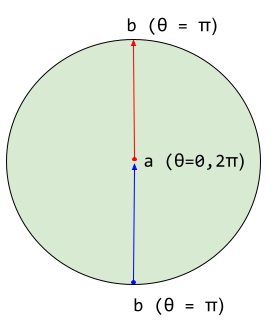
\includegraphics[width=0.4\textwidth]{RP3} \\[1em]
  lifts to these two paths in $\S^3$: $\angles{a_1,b_1,a_2}$ and $\angles{a_2,b_2,a_1}$.
  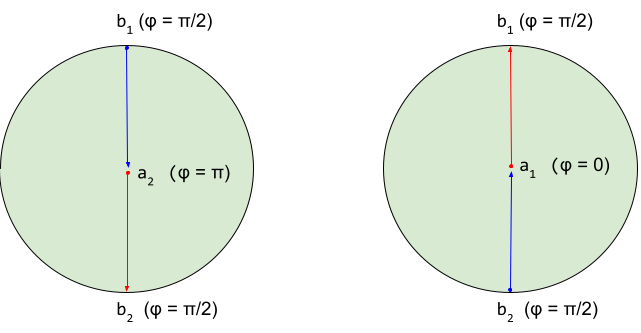
\includegraphics[width=0.9\textwidth]{S-3} \\
\end{tabular}








\bibliographystyle{amsalpha}
\bibliography{math}

\end{document}